% TODO: check spelling and grammar
\documentclass{article}
\usepackage{graphicx}

\begin{document}
\title{Syllabus - Psych 101, UC Berkeley, Summer 2018}
\author{Matthew J. Crossley}
\maketitle

\section{Instructor and GSI Information}
\begin{description}
\item [Instructor:] Matthew J. Crossley
  \begin{description}
  \item [email:] matthewjohncrossley@gmail.com
  \item [office:] TBA
  \item [office hours:] tues / thurs 12:00 - 1:00 or by appt.
  \end{description}

\item [GSI:] Felicia Zerwas
  \begin{description}
  \item [email:] fzerwas@berkeley.edu
  \item [office:] TBA
  \item [office hours:] TBA
  \end{description}

\item [GSI:] Joseph Ocampo:
    \begin{description}
  \item [email:] jmocampo@berkeley.edu
  \item [office:] TBA
  \item [office hours:] TBA
  \end{description}
\end{description}

\section{Course Schedule}
\begin{description}
\item [course date span:] June 18 to August 10
\item [lecture meeting times:] tues / thurs 9:00 - 11:30
\item [lecture meeting room:] Barrows 20
\item [section meeting time:] tues / thurs 1:00 - 3:00
\item [section meeting room:] TBA
\end{description}

\section{Website}
\begin{description}
\item[bcourses:] TBA
\item[github:] https://github.com/crossley/psych-101
\end{description}

\section{Course Information}
The goal of the course is to teach students basic statistics using the R
programming language. R will be at the very core of nearly everything we do.
Please make sure you have access to a reliable computer. Please also bring your
computer to lectures. You will learn much more, and help others by asking better
questions if you follow along with my programming examples during lecture.

\section{Prerequisites}
You must have a good grasp of algebra and be willing to try very hard to learn
the R programming language. Prior experience with R -- or similar language --
will be very helpful to you, but is not at all necessary. We will learn both
statistics and R from the ground up.

\section{Required Course Materials}
Students must have access to a computer that is successfully running the R
programming langauge.

\section{Course Composition and Grading Policy}
Your grade will be determined on the basis of your performance on 8 homework
assignments (1 per week of the course), and one final project. Each homework
assignment will be worth 100 points. The final project will be worth 800
points. Your final grade will be computed as follows:

\begin{figure}[h]
  \caption{Course grading algorithm.}
  \centering
    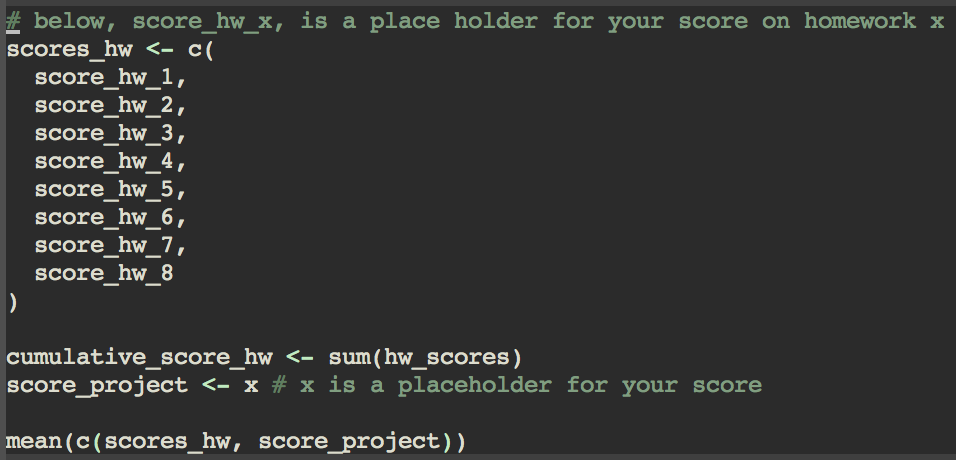
\includegraphics[width=0.9\textwidth]{final_grade}
\end{figure}


\section{Academic Honesty}
Both the University and your instructor take academic honesty very seriously. If
you are caught cheating on an exam or assignment, you will automatically fail
the class. This behavior will also be brought to the attention of the psychology
department and University. Afterward, further actions might then be taken by
both groups.

\section{Disability Statement}
If you are a student who needs academic accommodations or support because of a
documented disability, please contact me and provide copies of your contract
or accommodation letters within two weeks of the start of the semester. This
will allow me to make the appropriate arrangements. All discussions will remain
confidential. If you have questions about accessing Disability Support Services,
documenting a disability, or requesting accommodations, you should contact the
disability support program. More information can be found online.

\section{Student Learning Outcome and Course Requirements Met}
This course is required for the psychology major. It might also fulfill the
requirements for other majors. The class is required for majors because by the
end of this semester you should have gained: 1. The knowledge, understanding,
and critical thinking skills that are required in order to evaluate and
understand empirical work, and 2. The ability to effectively communicate your
logic and calculate out the statistics that you can and will use in experiments
during this semester and in future years.

\section{Disclaimer}
This syllabus is subject to modification. The instructor will communicate with
students on any changes.

\end{document}